\chapter{System Construction and Estimation}
\label{ch:system}

The modules of Chapter~\ref{ch:methods} are not yet a system. A passage has a camera, a trigger, a computer, a depth reading, and a person who has to act on a wrong tally. Section~\ref{sec:build} specifies that system around YOLO-vf-seg, ICPH, and PLC, at the level of geometry, data flow, calibration, timing, and the operator's record. Section~\ref{sec:estimate} then estimates the two modules under a Monte Carlo model whose parameters are the same numbers used in the specification. The estimate is a property of the model. It is the evidence this thesis can offer without a filmed passage, and the text keeps that limit visible next to every table.

\section{System construction}
\label{sec:build}

\subsection{The gate}
\label{sec:gate}

The system is installed at a warehouse door that every finished pallet passes, rather than on the forklift. A camera on the truck would move with the load and would see the load from a fixed relative pose, which is attractive, and it would require power, vibration isolation, and a radio on every truck, which this design refuses. A gate camera sees many trucks. The price is that the face is in view for a short interval, and that the interval depends on the driver.

The nominal installation is a camera whose optical axis is horizontal, at a height of $1.4\,\mathrm{m}$ above the floor, aimed perpendicular to the path of the truck at a standoff of about $2.5\,\mathrm{m}$ from the plane in which the front face is expected. At that standoff a face of width $1.6\,\mathrm{m}$, four nominal crates, subtends a moderate field of view, and a stack of six crates at $0.28\,\mathrm{m}$ reaches $1.68\,\mathrm{m}$ above the pallet. A pallet height of roughly $0.15\,\mathrm{m}$ puts the top of a six-high stack near $1.8\,\mathrm{m}$. The camera height of $1.4\,\mathrm{m}$ looks slightly down on the lower rows and slightly up at the top row, which is the perspective the homography is asked to remove. A camera placed at the top of the stack would see the top faces and would lose the bottom row to the pallet. A camera placed at fork height would see the forks and would clip the top. The middle of the design range is the compromise.

The shutter is specified from the truck speed rather than from a frame-rate fashion. At $1.5\,\mathrm{m\,s^{-1}}$, a walking pace, a $2\,\mathrm{ms}$ exposure moves the load by $3\,\mathrm{mm}$ during the exposure. That smear is small beside the $3.5\,\mathrm{cm}$ center noise already admitted in the lattice. At $5\,\mathrm{m\,s^{-1}}$ the same exposure moves the load by $10\,\mathrm{mm}$, still inside the half-cell of \Cref{prop:snap}, and a $10\,\mathrm{ms}$ exposure would move it by $50\,\mathrm{mm}$, which is a quarter of a cell and no longer negligible. The specification is therefore an exposure at or below $2\,\mathrm{ms}$, with the gain raised to compensate, and a frame rate of $15\,\mathrm{Hz}$ so that a face which is fully in view for half a second contributes about seven frames, of which the estimate's five-frame passage is a conservative subset. The blur variable in the observation model is the normalized version of whatever this exposure fails to prevent. It is not a second shutter design.

Illumination is not redesigned. The gate inherits the dock. What the system specifies instead is a prohibition and a calibration. The prohibition is against an automatic white balance in the camera firmware. Firmware white balance is a global gain of the kind Section~\ref{sec:color-principles} rejected, and it moves from frame to frame as the truck's painted mast enters the field. The camera is locked to a fixed gain and a fixed color balance for the shift. ICPH then sees a stable $\mathbf{L}$ inside the passage and a varying $\mathbf{L}$ between shifts, which is the variation the head was built for. The calibration is the weekly set of known-color pallets used to rank the margin, as in Section~\ref{sec:icph-margin}.

\subsection{What is computed, and where}
\label{sec:compute}

One industrial PC at the gate is sufficient. The segmenter is the heavy step. ICPH and PLC are not. A medium YOLO-seg model on a current embedded GPU sustains a frame rate above the $15\,\mathrm{Hz}$ of the camera if the input is kept near the model's training resolution; the warehouse result cited in Section~\ref{sec:warehouse-yolo}, $84.8$ frames per second for a small variant, is evidence that the family has margin, not a measurement of this PC. The design therefore budgets the segmenter at one frame period, the color head at well under a millisecond for a few dozen masks, and the lattice at well under a millisecond. The budget that can actually break is the segmenter. If a deployment finds that the medium model misses the frame period, the specified downgrade is a smaller YOLO-vf-seg variant with the same two heads, not the removal of PLC. Removing PLC reintroduces the factor-of-depth error, which is larger than the accuracy difference between a small and a medium backbone.

\begin{figure}[t]
\centering
\begin{tikzpicture}[
  font=\footnotesize,
  box/.style={draw, rounded corners=2pt, align=center, inner sep=3.5pt, minimum height=7mm},
  arr/.style={-{Stealth}, semithick}
]
  \node[box, fill=black!8] (cam) {Locked\\camera};
  \node[box, right=5mm of cam] (trig) {Passage\\trigger};
  \node[box, right=5mm of trig] (buf) {Frame\\buffer, $F{\le}7$};
  \node[box, right=5mm of buf] (yolo) {YOLO-vf-seg\\masks, centers};
  \node[box, fill=orange!15, below=6mm of yolo] (icph) {ICPH\\class, margin};
  \node[box, fill=green!12, left=5mm of icph] (pick) {Pick the\\sharp frame};
  \node[box, fill=green!12, left=5mm of pick] (plc) {PLC\\on that frame};
  \node[box, left=5mm of plc] (dep) {Depth\\reading $\hat{d}$};
  \node[box, fill=blue!8, below=6mm of pick] (rec) {Tally record\\per color and total};
  \draw[arr] (cam) -- (trig);
  \draw[arr] (trig) -- (buf);
  \draw[arr] (buf) -- (yolo);
  \draw[arr] (yolo) -- (icph);
  \draw[arr] (icph) -- (pick);
  \draw[arr] (pick) -- (plc);
  \draw[arr] (dep) -- (plc);
  \draw[arr] (plc) -- (rec);
  \draw[arr] (icph) -- (rec);
\end{tikzpicture}
\caption{Data flow of one passage. The camera's white balance is locked. The buffer holds a handful of frames. The segmenter runs on each. ICPH scores every mask. PLC runs once, on the frame the margins select. The depth reading joins only at the multiplication.}
\label{fig:dataflow}
\end{figure}

The software is a single process with the stages of \Cref{fig:dataflow}. The trigger is a motion detector or a break-beam at the gate; the design does not depend on which, provided the beam fires before the face is centered and holds the buffer open until the face has left. Frames that fail a coarse brightness check are dropped rather than segmented. On each kept frame the segmenter writes masks, boxes, and centers. ICPH writes a class and a margin per mask. When the trigger closes, the frame with the highest median margin is passed to PLC together with the depth reading. The record in Section~\ref{sec:sys-output} is written once. There is no tracking identity across frames in the specified system. Section~\ref{sec:plc-passage} is why: a union of cells made the count worse under the model, and the software does not implement a method the estimate has already rejected.

The depth reading arrives on a separate path. The preferred source is the pallet build record, if the packaging line already knows whether it stacked one, two, or three deep. The fallback is a manual default for the shift, displayed as a default so that the uncertainty triple of Section~\ref{sec:plc-uncertainty} has its depth bit clear. The system does not infer depth from the side masks. That constraint is enforced in the software by the absence of any code path from the mask area to $\hat{d}$.

\subsection{The segmenter as a component}
\label{sec:segmenter-component}

YOLO-vf-seg is used as specified in Section~\ref{sec:problem-gap}. The input is a three-channel image at the network's native resolution. The neck applies the vertical-feature gate~\eqref{eq:vf} on the three pyramid levels that feed the head. The detection head emits boxes and objectness. The mask head emits thirty-two prototypes and a coefficient vector per detection, combined by~\eqref{eq:yolact} and cropped to the box. Non-maximum suppression keeps one detection per crate when the boxes overlap heavily. The suppression threshold is part of the deployment calibration, not part of the Monte Carlo model. The model represents a miss by a detection probability that already folds suppression, shadow, and blur into one number. A future measurement on real frames would have to unfold that number before anyone tuned the suppression threshold against this thesis's tables.

The segmenter is not trained in this thesis. A deployment train would start from a public YOLO-seg checkpoint trained on COCO~\cite{lin2014coco,jocher2023yolov8} and would continue on gate images labeled for masks and for the six colors. The color labels are the same labels ICPH needs, so one labeling pass serves both the mask head's class branch and the chromatic head. The vertical-feature gate can be trained from the start or folded in after the baseline converges. Neither schedule is estimated here. What the system specification fixes is the interface the training must preserve: masks whose first moment is a usable center, and pixels inside the mask that are still the crate's pixels. A training run that inflates masks to win a region overlap will hand ICPH the neighbor's color and will hand PLC a center that has drifted toward the neighbor. The overlap loss is therefore not the only training criterion a deployment should watch. The center error in centimetres on the rectified face, the quantity \Cref{prop:snap} bounds, is the criterion that matches the lattice.

\subsection{Calibration}
\label{sec:calibration}

Three calibrations are specified, and they are not optional in the way a software default is optional.

The geometric calibration estimates $K$ and $H$. A planar target of known spacing is held in the plane of a typical front face, the camera is locked, and $H$ is computed by the direct linear transform with RANSAC rejection of corners that the detector mismatched~\cite{zhang2000calibration,hartley2004mvg,fischler1981ransac}. The scale of $H$ is fixed by the target, in metres. After calibration, a person checks that the residual of a crate-sized rectangle on the target is small beside $w/2$. This calibration is repeated when the camera moves. A temperature drift of a fixed camera is ignored until that residual, checked at the start of a week, grows.

The pitch calibration is a confirmation, not an estimation. The nominal $(w,h)=(0.40,0.28)\,\mathrm{m}$ is checked with a tape on the crate family that the gate will see. If a second family is present, its pitch is entered as a second hypothesis. The origin estimator~\eqref{eq:origin} then runs twice and the hypothesis with the smaller median absolute residual is kept. The estimate in Section~\ref{sec:estimate} uses one pitch. The second hypothesis is specified so that the software has a place to put it, and so that nobody ``solves'' a second family by stretching $H$.

The color calibration is the weekly set of known pallets. It does not refit $W$. It records the distribution of margins and sets the abstention threshold at the tenth percentile of that distribution, as Section~\ref{sec:icph-margin} states. Refitting $W$ is a maintenance action, taken when the abstention rate rises for a week, not a per-passage action. Refitting on the passage itself would let a single badly lit truck move the prototypes.

\subsection{Timing inside one passage}
\label{sec:timing}

\begin{table}[t]
\centering
\caption{Timing budget for one passage at $15\,\mathrm{Hz}$ with five kept frames. The segmenter line is a budget, not a measured latency of a named device. The other lines are consequences of the algorithms in Chapter~\ref{ch:methods}.}
\label{tab:timing}
\small
\begin{tabular}{@{}lcc@{}}
\toprule
Stage & When & Budget \\
\midrule
Exposure and readout & every frame & $\le 2\,\mathrm{ms}$ exposure \\
YOLO-vf-seg & every kept frame & one frame period \\
ICPH, all masks of the frame & every kept frame & $<1\,\mathrm{ms}$ \\
Sharp-frame selection & trigger close & negligible \\
Homography on the centers & once & negligible \\
PLC origin, snap, completion & once & negligible \\
Write the tally record & once & negligible \\
\bottomrule
\end{tabular}
\end{table}

\Cref{tab:timing} is a budget that makes the dependence explicit. The system is late if and only if the segmenter is late, or if the trigger opens so late that fewer than one sharp frame is buffered. Both of those failures are detectable. A late segmenter drops a frame and still returns a tally from the frames it finished. An empty buffer returns no tally and an explicit failure, rather than a zero count. A zero count is a legal tally of an empty pallet and must not be reused as the code for ``the camera blinked.''

\subsection{The record the operator sees}
\label{sec:sys-output}

The record of a passage contains one line per color and one total, plus the diagnostics that change the meaning of those numbers. The fields are:

\begin{enumerate}
\item time, gate identity, and the frame index that PLC used;
\item $\hat{N}_{k}$ for each color, computed by~\eqref{eq:per-color}, with uncertain masks listed separately and not folded into a color;
\item the total $\hat{N}=\hat{d}\,\lvert\mathcal{F}\rvert$;
\item the depth reading and whether it was a default;
\item the number of completed cells $\lvert\mathcal{F}\setminus\mathcal{D}\rvert$;
\item the median origin residual, in centimetres;
\item the minimum color margin on the chosen frame.
\end{enumerate}

A total without the completed-cell count would hide the difference between a stack that was seen and a stack that was inferred. A per-color tally without the minimum margin would hide an amber--yellow swap. The seven fields are the smallest set that matches the failure modes of \Cref{fig:failures}. The display does not show a live mask overlay as a requirement. An overlay is useful during calibration and is not part of the tally the warehouse books.

Fault handling is a list of refusals. The system refuses to book a total when the buffer is empty, when the origin residual exceeds half a cell, or when $\hat{d}$ is missing and no shift default exists. In each refusal the images are kept and the passage is marked for a person. The system does not refuse merely because a margin is low. It books the total, withholds the uncertain color, and says so. That split follows from the independence of the two modules: a bad color is not a bad count.

\subsection{What the construction deliberately leaves out}
\label{sec:leave-out}

No second camera is specified. No truck-mounted computer is specified. No automatic white balance is permitted. No density branch is added to the segmenter. No multi-frame union is used in the tally. Each omission corresponds to a result or a requirement already stated. Listing them here is part of the construction, because a later implementer who adds a union ``for robustness'' would be reversing Section~\ref{sec:plc-passage} without a new measurement. The place to revisit any of these omissions is a field trial that measures the corresponding error, not a default setting in the process.

The construction is complete enough to implement and incomplete in the way any unfilmed design is incomplete. It does not name a lens, a cable, or a model of PC. Those are procurement choices inside the geometric and timing constraints above. The constraints are the design.

\section{Estimation}
\label{sec:estimate}

\subsection{Status of the numbers}
\label{sec:status}

Every number in this section comes from one instrument, \texttt{simulate\_estimation.py}, run at a fixed seed, writing \texttt{estimation\_results.json}. The instrument implements the observation models of Sections~\ref{sec:color-model} and~\ref{sec:count-model}. It does not read an image. It does not fine-tune a detector. A table below is therefore an estimate of a module under a stated generative model. Where the model is harsh, the estimate is harsh. Where the model omits a nuisance, the estimate is silent on that nuisance. The discussion in Section~\ref{sec:reading} says which silences matter.

The instrument has two independent blocks. The color block trains the linear ICPH of~\eqref{eq:linear} and tests it against raw cosine matching, gray-world, and shades-of-gray. The counting block does not look at color. It drops centers with a position-dependent probability, snaps the survivors, and scores six counters. Independence is a modeling choice already used in~\eqref{eq:bound}. It means the tables must not be multiplied together into a single invented accuracy.

\subsection{Observation model for color}
\label{sec:color-model}

A test patch is drawn by the same steps as training, with the severity held fixed so that a curve against illuminant strength exists. The severity values are $0.05$, $0.15$, $0.30$, $0.45$, and $0.60$. At each value, $2500$ patches are drawn, the class uniform on the six prototypes, the gain as in~\eqref{eq:gain} with that fixed $s$, the shadow, the shade ramp, the neighbor strip with probability $0.25$, and the pixel noise. Training used $6000$ patches with $s$ random in $[0.05,0.55]$ and $500$ full-batch steps at learning rate $0.35$ and $\lambda=10^{-3}$. Test patches are not in the training set; they are fresh draws, which for this generator is the relevant notion of ``unseen.''

The four decision rules are exactly those of Section~\ref{sec:icph-score}. Raw matching uses~\eqref{eq:raw} on the uncorrected mean. Gray-world corrects with $p=1$ and then matches. Shades-of-gray corrects with $p=6$ and then matches. ICPH computes~\eqref{eq:feature}, standardizes with the training moments, and applies the trained $W$ and $b$. Accuracy is the fraction of patches whose predicted class equals the class that generated the reflectance, before the illuminant was applied. A neighbor strip does not change the label. The label is the class of the face that owns the patch, not the class of the contaminating strip. That choice makes boundary error count against the classifier, which is the deployment meaning of a messy mask.

\subsection{Observation model for counting}
\label{sec:count-model}

A trial draws a stack and then a noisy view of it. The number of front rows is uniform on $\{2,3,4,5,6\}$, the number of columns uniform on $\{2,3,4\}$, and the depth uniform on $\{1,2,3\}$. Each front cell is occupied with probability $0.93$, and the stack is forced to contain at least one crate. A blur variable $\beta$ is uniform on $[0,1]$. The probability that an occupied cell is detected is
\begin{equation}
\pi(r)
= \operatorname{clip}\!\big(\pi_0(r)-0.18\,\beta,\, 0.35,\, 0.99\big),
\label{eq:detprob}
\end{equation}
with $\pi_0=0.70$ on the bottom row, $0.84$ on the top row, $0.96$ on a middle row, and $0.90$ if the stack has only one row. A detected center is the cell center plus independent Gaussian noise of standard deviation $0.035\,\mathrm{m}$ in $x$ and $0.028\,\mathrm{m}$ in $y$. A Poisson number of false centers, mean $0.35$, is thrown uniformly into a rectangle slightly larger than the stack. Depth is observed by~\eqref{eq:depth}. Five frames are drawn independently for each trial. Four thousand trials are run.

The six counters are the mask tally~\eqref{eq:mask-count}, the mask tally times depth, the area ratio~\eqref{eq:area}, the span~\eqref{eq:span}, PLC on the first frame, and PLC on the union of the five frames with vote threshold one. The area-ratio fraction and the span percentile match Section~\ref{sec:plc-baselines}. PLC matches \Cref{alg:plc}. The truth is~\eqref{eq:true-count}.

\subsection{Metrics}
\label{sec:est-metrics}

Color uses top-1 accuracy at each severity, plus, at the harshest severity, the per-class recall and the full confusion matrix of ICPH. Counting uses, for each counter, the mean absolute error, the root mean square error, the signed bias, the fraction of trials with an exact total, the mean absolute percentage error, and the ninetieth percentile of the absolute error. Errors are $\hat{N}-N$, so a negative bias is a counter that is short. The same absolute and squared errors are broken out by true depth, because a counter that ignores depth will look acceptable at depth one and unacceptable at depth three. The mean true count in the four thousand trials is $22.62$ with standard deviation $14.57$, which is the denominator that makes a mean absolute error of three crates a relative error of roughly one seventh, not a small or a large number by itself.

\subsection{Color results}
\label{sec:color-results}

\begin{table}[t]
\centering
\caption{Top-1 color accuracy on $2500$ patches at each illuminant severity. Gray-world uses $p=1$. Shades-of-gray uses $p=6$. ICPH is the linear head on the eight-dimensional feature. The generator, not a photographed aisle, produced the patches.}
\label{tab:color}
\small
\begin{tabular}{@{}lcccc@{}}
\toprule
Severity $s$ & Raw RGB & Gray-world & Shades-of-gray & ICPH \\
\midrule
$0.05$ & $0.986$ & $0.165$ & $0.196$ & $0.972$ \\
$0.15$ & $0.900$ & $0.180$ & $0.211$ & $0.914$ \\
$0.30$ & $0.778$ & $0.186$ & $0.219$ & $0.834$ \\
$0.45$ & $0.618$ & $0.172$ & $0.208$ & $0.687$ \\
$0.60$ & $0.531$ & $0.171$ & $0.204$ & $0.607$ \\
\bottomrule
\end{tabular}
\end{table}

\begin{figure}[t]
\centering
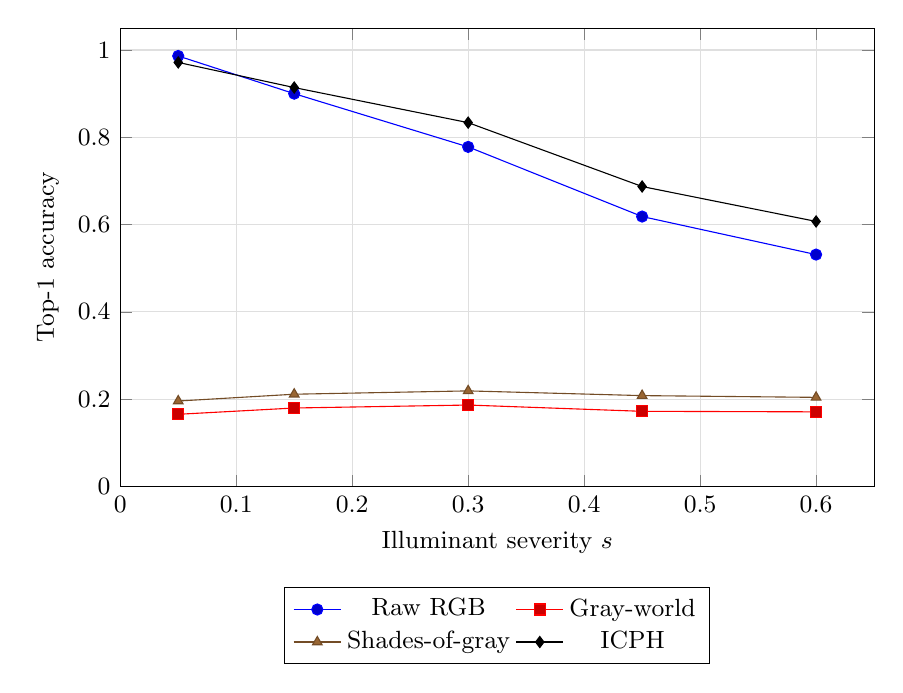
\begin{tikzpicture}
\begin{axis}[
  width=0.92\textwidth,
  height=7.4cm,
  xlabel={Illuminant severity $s$},
  ylabel={Top-1 accuracy},
  ymin=0, ymax=1.05,
  xmin=0, xmax=0.65,
  legend style={font=\small, at={(0.5,-0.22)}, anchor=north, legend columns=2},
  tick label style={font=\small},
  label style={font=\small},
  grid=major,
  grid style={gray!25}
]
\addplot+[mark=*] coordinates {(0.05,0.9864) (0.15,0.9000) (0.30,0.7780) (0.45,0.6184) (0.60,0.5312)};
\addplot+[mark=square*] coordinates {(0.05,0.1652) (0.15,0.1796) (0.30,0.1864) (0.45,0.1720) (0.60,0.1708)};
\addplot+[mark=triangle*] coordinates {(0.05,0.1956) (0.15,0.2112) (0.30,0.2188) (0.45,0.2080) (0.60,0.2040)};
\addplot+[mark=diamond*] coordinates {(0.05,0.9716) (0.15,0.9140) (0.30,0.8336) (0.45,0.6872) (0.60,0.6072)};
\legend{Raw RGB, Gray-world, Shades-of-gray, ICPH}
\end{axis}
\end{tikzpicture}
\caption{The same numbers as \Cref{tab:color}. Classical correction sits near chance for every severity. Raw matching wins only while the lamp is nearly white. ICPH degrades more slowly once the severity leaves that regime.}
\label{fig:color-curve}
\end{figure}

\Cref{tab:color} and \Cref{fig:color-curve} match the contract of Section~\ref{sec:icph-cost}. Gray-world and shades-of-gray stay between $0.165$ and $0.219$ at every severity. Chance on six classes is $0.167$. \Cref{prop:uniform} said a uniform face would be driven to neutral by the correction, and a face that is only mildly contaminated is not driven all the way, which is why the two classical rules sit just above chance rather than on it. They do not become more accurate as the illuminant grows, because the destruction of reflectance happens before the illuminant is interesting.

Raw matching at $s=0.05$ reaches $0.986$, above ICPH at $0.972$. That crossover was predicted: when the gain is almost white, dividing by $\hat{\ell}$ spends a clean reflectance signal to buy an illuminant correction that was unnecessary. By $s=0.15$ the order has reversed, $0.914$ against $0.900$. The gap then widens and stays modest: $0.056$ at $s=0.30$, $0.069$ at $s=0.45$, and $0.076$ at $s=0.60$. ICPH at the harshest setting is $0.607$, which is better than raw and far from solved. A deployment that sees lamps of this severity will abstain often, which is why the margin rule exists. The curve does not support a claim that the chromatic feature has removed illumination.

\begin{table}[t]
\centering
\caption{Confusion matrix of ICPH at severity $0.60$. Rows are the true class, columns the predicted class, in the order amber, green, red, blue, yellow, white. Each row sums to the number of test patches of that class inside the $2500$.}
\label{tab:confusion}
\small
\begin{tabular}{@{}lrrrrrr@{}}
\toprule
True $\backslash$ predicted & amber & green & red & blue & yellow & white \\
\midrule
amber  & 171 & 15 & 43 & 0 & 118 & 19 \\
green  & 4 & 271 & 2 & 51 & 33 & 46 \\
red    & 53 & 1 & 321 & 2 & 6 & 29 \\
blue   & 0 & 48 & 0 & 361 & 0 & 38 \\
yellow & 130 & 54 & 41 & 0 & 179 & 37 \\
white  & 21 & 66 & 34 & 70 & 21 & 215 \\
\bottomrule
\end{tabular}
\end{table}

\Cref{tab:confusion} is the harsh-severity detail behind the mean of $0.607$. Per-class recall is $0.467$ for amber, $0.666$ for green, $0.779$ for red, $0.808$ for blue, $0.406$ for yellow, and $0.504$ for white. Amber sends $118$ patches to yellow, and yellow sends $130$ patches to amber. That pair is the failure named in Section~\ref{sec:icph-cost}, and it is large enough that a mean accuracy which hides it would be a misleading summary. Red and blue are the classes the feature can hold. White's errors are spread across all five chromatic classes, $21$, $66$, $34$, $70$, and $21$, which is the neutral-axis prediction and not a single swap. Green leaks toward blue and white more than toward red, consistent with a prototype that already sits between those neighbors in \Cref{fig:chroma-plane}.

The operating consequence is narrower than ``use ICPH.'' Under a mild lamp, raw matching is enough and slightly better. Under a lamp the weekly calibration shows to be strong, ICPH is the better of the two and still needs the abstention rule, aimed first at amber and yellow. Under either lamp, a corrected-then-matched baseline is not a competitor. It is a demonstration of \Cref{prop:uniform}.

\subsection{Counting results}
\label{sec:count-results}

\begin{table}[t]
\centering
\caption{Counting error on $4000$ stacks. Bias is the mean of $\hat{N}-N$. Exact is the fraction of trials with $\hat{N}=N$. PLC-single uses the first frame. PLC-passage unions five frames at vote one. The mean true count is $22.62$.}
\label{tab:count}
\small
\begin{tabular}{@{}lrrrrrr@{}}
\toprule
Counter & MAE & RMSE & Bias & Exact & MAPE & P90 $\lvert e\rvert$ \\
\midrule
Mask, no depth & $13.55$ & $18.04$ & $-13.53$ & $0.044$ & $0.517$ & $31$ \\
Mask $\times$ depth & $4.87$ & $6.69$ & $-4.33$ & $0.126$ & $0.229$ & $12$ \\
Area ratio & $7.26$ & $9.19$ & $-7.08$ & $0.030$ & $0.328$ & $15$ \\
Span lattice & $3.31$ & $5.50$ & $+1.60$ & $0.332$ & $0.178$ & $9$ \\
PLC-single & $3.01$ & $5.00$ & $+0.83$ & $0.337$ & $0.162$ & $8$ \\
PLC-passage & $5.80$ & $8.79$ & $+5.33$ & $0.221$ & $0.318$ & $15$ \\
\bottomrule
\end{tabular}
\end{table}

\begin{figure}[t]
\centering
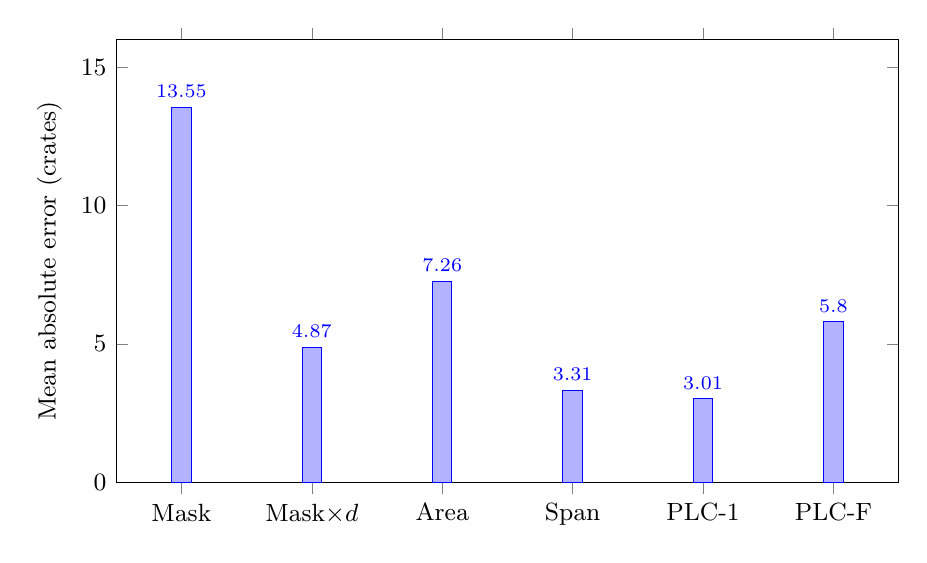
\begin{tikzpicture}
\begin{axis}[
  width=0.95\textwidth,
  height=7.2cm,
  ybar,
  bar width=7pt,
  ylabel={Mean absolute error (crates)},
  symbolic x coords={Mask,Mask$\times d$,Area,Span,PLC-1,PLC-F},
  xtick=data,
  x tick label style={font=\small},
  y tick label style={font=\small},
  ymin=0, ymax=16,
  nodes near coords,
  every node near coord/.append style={font=\scriptsize, /pgf/number format/fixed},
  label style={font=\small}
]
\addplot coordinates {(Mask,13.55) (Mask$\times d$,4.87) (Area,7.26) (Span,3.31) (PLC-1,3.01) (PLC-F,5.80)};
\end{axis}
\end{tikzpicture}
\caption{Mean absolute error of the six counters, from \Cref{tab:count}. The vertical axis is crates per passage, on a mean load of about $23$ crates. PLC on one frame is the lowest bar. The five-frame union is not.}
\label{fig:count-bars}
\end{figure}

\Cref{tab:count} is the counting claim of Section~\ref{sec:plc-claims}, measured. The mask tally without depth has bias $-13.53$ and mean absolute error $13.55$. The two numbers are almost equal, which means the error is nearly a pure under-count: the tally sees the front and the truth includes the ranks behind it. Multiplying the same masks by $\hat{d}$ cuts the mean absolute error to $4.87$ and the bias to $-4.33$. Depth is the dominant correction. Any discussion of lattice refinement that omits this comparison will attribute to geometry what belongs to the integer $\hat{d}$.

Given depth, the area ratio is worse than the raw mask count, $7.26$ against $4.87$, with bias $-7.08$. The visible-fraction model has mean $0.86$. Summing fractions that are systematically below one, then rounding, short-changes a stack whose detections were already a little short. The area ratio would need a fraction model centered on one, or a completion rule of its own, before it could be the inventory method of Hu, Wang, and Yang~\cite{hu2025arbca} inside this generator. The comparison does not refute that paper's measurement on tobacco cargo. It shows that a fraction below one is the wrong summary of a missed crate of known size.

The span and PLC-single are the two counters that use the pitch. Span reaches mean absolute error $3.31$, bias $+1.60$, exact on $0.332$ of trials. PLC-single reaches $3.01$, bias $+0.83$, exact on $0.337$. The absolute-error gap is three tenths of a crate on a load of about twenty-three. The bias gap is the clearer signature of the gap rule: both methods over-fill, and the two-neighbor rule over-fills less than the solid rectangle of the span. Neither is exact on a majority of trials. A ninetieth percentile of eight crates for PLC-single is a large tail. The tail is where the depth reading is off by one, because a wrong rank costs $\lvert\mathcal{F}\rvert$ crates at once, or where the outline is a step that completion fills.

PLC-passage is the negative result. Mean absolute error $5.80$, bias $+5.33$, exact on $0.221$. The bias and the absolute error are close, so the passage union is a nearly pure over-count, as Section~\ref{sec:plc-passage} argued from the vote threshold of one. Five frames are worse than one frame. The system specification that runs PLC once is this row of the table, not a preference for simpler code.

\begin{table}[t]
\centering
\caption{Mean absolute error by true depth. The number of trials is $1326$, $1329$, and $1345$ at depths $1$, $2$, and $3$.}
\label{tab:bydepth}
\small
\begin{tabular}{@{}lrrr@{}}
\toprule
Counter & Depth $1$ & Depth $2$ & Depth $3$ \\
\midrule
Mask, no depth & $2.27$ & $13.30$ & $24.93$ \\
Mask $\times$ depth & $2.50$ & $4.89$ & $7.18$ \\
Area ratio & $3.53$ & $7.22$ & $10.98$ \\
Span lattice & $1.91$ & $3.59$ & $4.40$ \\
PLC-single & $1.72$ & $3.27$ & $4.03$ \\
PLC-passage & $3.29$ & $5.96$ & $8.12$ \\
\bottomrule
\end{tabular}
\end{table}

\Cref{tab:bydepth} separates the depth effect. The mask tally's error scales almost exactly with the hidden ranks: $2.27$, $13.30$, $24.93$. At depth one it is competitive with the geometric counters, because there is no hidden rank and the remaining error is detection noise. At depth three it is an inventory error of a different kind. Mask times depth grows much more slowly, $2.50$, $4.89$, $7.18$, and the growth is the combination of front-face misses scaled by $\hat{d}$ and the ten percent of trials in which $\hat{d}$ itself is wrong. PLC-single is the best entry in every column: $1.72$, $3.27$, $4.03$. The margin over the span is small and has the same sign in every column, which is what a refinement rather than a different estimator looks like. PLC-passage is worse than PLC-single in every column, so the over-fill is not an artifact of one depth.

Bias, not shown in that table and computed in the same run, stays negative for the mask and the area ratio at every depth, and stays positive for the span and both PLC variants at every depth. The sign flip between ``count what you saw'' and ``complete a lattice'' is stable across the design range. An operator who trusts PLC is accepting a small positive bias in exchange for a smaller absolute error. The completed-cell field on the record is the way that acceptance is made visible per passage rather than only in a table of four thousand trials.

\subsection{One passage, computed by hand and by the instrument}
\label{sec:one-passage}

One draw in the run has the front occupancy~\eqref{eq:example-grid}, depth $2$, and therefore truth $20$. The blur draw is $0.161$. The five frames contain $9$, $10$, $10$, $10$, and $10$ detections. The first frame is one short of the ten true front cells. PLC on that frame returns $22$. The span on that frame returns $24$. The mask tally returns $9$, which is the front count with one miss and no depth. PLC-passage on all five frames returns $28$.

Section~\ref{sec:plc-example} already accounts for the $22$: one missed cell put back by the neighbor rule, one phantom cell added on the stepped top row, eleven front cells times depth $2$. The span's $24$ is the bounding rectangle, three columns by four rows, times depth $2$, which fills both empty cells of the top row rather than one of them. The passage result of $28$ is fourteen front cells times depth $2$, four cells above the truth on the front face. Those four are the union's contribution. The instrument and the hand rule agree on the frame that was short, which is the check that \Cref{alg:plc} in the text and the instrument are the same algorithm. They do not agree with the truth. The example is a picture of the positive bias, chosen because the grid is small enough to count, not because the error is flattering.

\subsection{Parameter cost of the head}
\label{sec:cost-result}

The cost model of~\eqref{eq:params} is a count of weights, not a profiled runtime. The reference segmenter in that model is a YOLOv8m-seg scale network, $27.3$ million parameters and on the order of $10^{2}$ GFLOPs, whose published COCO box and mask figures sit near $50$ and $41$ mean average precision. Those COCO figures are a reference for the size of the network. They are not a prediction of gate accuracy. On top of that network the specified ICPH adds $9760$ parameters, a fraction of $3.6\times 10^{-4}$. The counting stage adds none. The estimate of accuracy and the estimate of cost answer different questions. The cost answer is that the color head is not the part of the system a deployer would shrink first. The accuracy answer is that the head is worth having when the illuminant is not mild, and that it does not resolve amber against yellow at severity $0.60$.

\subsection{How to read the estimate}
\label{sec:reading}

The estimate supports five statements, and it does not support a sixth.

It supports the statement that classical per-mask color constancy is the wrong correction on a nearly uniform crate face. That statement is \Cref{prop:uniform} plus the flat curves near chance in \Cref{fig:color-curve}. It does not depend on the linear head being optimal.

It supports the statement that a linear head on $(\chi,o,\eta)$ degrades more slowly than raw cosine matching as the illuminant severity grows, and that the residual errors concentrate on amber, yellow, and white. The crossover at low severity is part of the statement, not a footnote.

It supports the statement that multiplying a front count by a depth reading is the largest single reduction in counting error available inside this model. The reduction from $13.55$ to $4.87$ mean absolute error dominates the later geometric refinements.

It supports the statement that, given depth, a lattice snap with two-neighbor completion is a small improvement on a span fill and a clear improvement on an area ratio whose visible fraction averages below one. The improvement is a few tenths of a crate on the mean, and a reduction of positive bias.

It supports the statement that unioning five frames at a vote of one increases positive bias. The recommended system runs PLC on one frame because of this statement, not in spite of it.

It does not support a field accuracy, a claim about cardboard of unknown pitch, a claim about a different depth-sensor error rate, or a claim that the neck path of Section~\ref{sec:icph-neck} has been trained. Those would require images, a second pitch, a measured sensor, and a trained backbone. The instrument does not contain them, and the tables do not imply them.

A reader who needs a single comparison should take it from \Cref{tab:count} and \Cref{tab:color} together and keep the conditions attached. At severity $0.30$, ICPH names the design palette correctly on about five patches in six, against about four in five for raw matching and about one in five for a classical correction. On the counting model, PLC-single is off by about three crates on a load of about twenty-three, against about five for masks times depth and about fourteen for masks alone. Both sentences are about the generators in Sections~\ref{sec:color-model} and~\ref{sec:count-model}.

\subsection{What a field trial would have to add}
\label{sec:field}

A trial that could replace this estimate would record, at one gate, the images, the depth reading, a person-confirmed count per color, and the lamp condition in enough variety that severity has an empirical meaning. It would report the same metrics: signed bias, exact total, exact per-color count, and abstention rate. It would keep PLC-single and PLC-passage as separate rows, because the passage result is easy to ``improve'' by a code change that the model has already rejected. It would publish the confusion matrix, not only the mean, because amber and yellow can move the mean by a point while dominating the inventory complaints.

Until that trial exists, the system of Section~\ref{sec:build} is a specification and the tables of this section are an estimate of its two numerical modules. The specification is already constrained by the estimate: one frame, not five; a chromatic feature, not a corrected color; depth as an input, not as a fraction of mask area. That is the sense in which the estimation chapter closes the design. It does not close the measurement.

\subsection{Footprint of a pixel on the crate face}
\label{sec:footprint}

The timing budget and the snap radius should be checked against the size of a pixel, otherwise the centimetre noise in the observation model is an unattached number. Take the installation of Section~\ref{sec:gate}: standoff $Z=2.5\,\mathrm{m}$, face width of interest $1.6\,\mathrm{m}$ for four crates, and a sensor used in landscape orientation. A horizontal field of view of $50^{\circ}$ covers
\begin{equation}
2\,Z\tan(25^{\circ}) = 2\cdot 2.5\cdot 0.466 = 2.33\,\mathrm{m}
\label{eq:fov}
\end{equation}
at the front plane, which leaves margin around a $1.6\,\mathrm{m}$ face for a truck that is not perfectly centered. Across $1280$ horizontal pixels the footprint is
\begin{equation}
\frac{2.33}{1280} = 1.8\,\mathrm{mm}
\label{eq:footprint}
\end{equation}
per pixel at the center of the field. The vertical footprint is comparable near the camera height and larger toward the top and bottom rows, where the ray is oblique. A center error of one pixel is negligible beside the $3.5\,\mathrm{cm}$ localization noise of the model and beside the $20\,\mathrm{cm}$ half-cell of \Cref{prop:snap}. The lattice is not limited by sensor resolution at this standoff. It is limited by which crates are detected and by whether the homography scale is right.

The same footprint converts the exposure specification into pixels of smear. At $1.5\,\mathrm{m\,s^{-1}}$ and $2\,\mathrm{ms}$ the load moves $3\,\mathrm{mm}$, about two pixels. At $5\,\mathrm{m\,s^{-1}}$ and $2\,\mathrm{ms}$ it moves $10\,\mathrm{mm}$, about six pixels. Six pixels of horizontal smear on a vertical lip, which is the lip the vertical-feature gate is trying to see, is a loss of contrast rather than a displacement of the center by a full cell. The $2\,\mathrm{ms}$ exposure is the specification that keeps smear in that regime. A camera that cannot reach it at the illumination of the dock has to add light. The design does not respond to a dark dock by lengthening the shutter, because the snap radius is a counting requirement and the brightness is a procurement requirement.

\begin{figure}[t]
\centering
\begin{tikzpicture}[x=0.72cm,y=0.72cm,font=\small]
  \draw[thick] (0,0) -- (14,0);
  \draw[dashed] (2,0) -- (2,6.2) node[above] {\footnotesize truck path};
  \draw[dashed] (8.2,0) -- (8.2,6.2);
  \node[align=center] at (5.1,5.6) {\footnotesize front-face plane};
  \draw[{Stealth}-{Stealth}] (2,5.1) -- (8.2,5.1) node[midway, above] {$2.5\,\mathrm{m}$};
  \draw[fill=black!80] (10.6,2.4) rectangle (11.7,3.1);
  \draw[-{Stealth}, thick] (10.6,2.75) -- (8.2,2.75);
  \node[align=center] at (11.15,3.55) {\footnotesize camera\\[-1pt]\footnotesize $1.4\,\mathrm{m}$};
  \draw[{Stealth}-{Stealth}] (12.3,0) -- (12.3,2.75) node[midway, right] {\footnotesize $1.4\,\mathrm{m}$};
  \draw[fill=orange!30] (4.3,0.4) rectangle (5.9,3.6);
  \node[align=center] at (5.1,2.0) {\footnotesize stack};
  \node[align=center] at (5.1,-0.55) {\footnotesize gate floor};
\end{tikzpicture}
\caption{Plan-and-elevation sketch of the gate, not to a common scale. The camera is fixed, the face plane is the calibration plane of $H$, and the standoff is the $Z$ used in~\eqref{eq:fov}. The truck path is perpendicular to the optical axis at the moment PLC is meant to run.}
\label{fig:gate}
\end{figure}

\subsection{From pixels to a booked line}
\label{sec:booked-line}

The pieces are scattered through the derivations. One passage, with the numbers of the worked example, shows the order in which the computer applies them. The trigger opens. Five frames are buffered. On each frame YOLO-vf-seg emits masks. ICPH scores each mask. Suppose the first frame has the lowest blur and the highest median margin, and that its ten true front crates produced nine detections, as in the instrument's draw. The nine centers are multiplied by $H$ and snapped. The origin residual is a few centimetres, inside the half-cell, so the passage is not refused. The gap rule adds the restored miss and the one phantom cell of \Cref{fig:grid}. The depth reading returns $2$, which matches the truth in this particular draw. The total booked is $11\times 2=22$ against a truth of $20$. The completed-cell count is $2$ if both the restored cell and the phantom were absent from the raw snap, and the record shows that $2$. The color head names the nine detected faces. The two cells that were not detected inherit by~\eqref{eq:per-color}. If one of the nine was an amber face scored as yellow with a margin below the weekly tenth percentile, that face is listed as uncertain and is not forced into either color's tally, while the total stays $22$.

The operator who sees this record can do three different things, and the record is built so that they stay different. A total of $22$ with two completed cells and a small residual is a geometric inference, to be trusted to the extent the building trusts PLC-single's bias of under one crate on average. An uncertain amber is a color question, to be confirmed from the image or from the pallet ticket, without reopening the total. A depth field that says ``default'' rather than ``from the pallet record'' is a rank question. Collapsing all three into a red flag would send every stepped stack to a person. Separating them sends the person the question the model cannot answer.

The same passage under the counters that were rejected reads as follows. The mask tally books $9$ and is short by $11$, because it ignores depth and one miss. Mask times depth books $18$ and is short by $2$. The span books $24$, the full rectangle times depth, and is long by $4$. PLC-passage, given the instrument's five detection counts of $9,10,10,10,10$, books $28$ and is long by $8$. The booked line of the specified system is the least wrong of those integers on this draw, and it is still wrong by two crates. The worked passage is not a demonstration that the error has been removed. It is a demonstration that the record contains the integer and the reason the integer might be high.

\subsection{Sensitivity to the depth reading}
\label{sec:depth-sensitivity}

The depth model fixes a ten percent chance of being off by one. The tables do not vary that chance, and a reader will want the direction of the dependence. Condition on the front estimate $\lvert\mathcal{F}\rvert$ being some integer $m$, and on the truth $N=d\,m_{\star}$. When $\hat{d}=d$, the counting error is $d(m-m_{\star})$, the front error scaled by depth. When $\hat{d}=d+1$, the error gains an extra $m$. When $\hat{d}=d-1$, it loses $m$. At the stated probability $0.10$ of a wrong reading, split equally between the two directions and ignoring the clip at the ends of $\{1,2,3\}$, the expected contribution of depth noise alone is of order $0.1\,m$ in absolute error and near zero in bias, because the two directions cancel in the signed mean and add in the absolute mean. On a front of about ten cells, depth noise contributes on the order of one crate of mean absolute error. That is a substantial part of PLC-single's $3.01$, and it is a part no lattice rule can remove.

Two consequences follow for the building, both outside the Monte Carlo grid and both readable from the scaling. Halving the depth error rate, from $0.10$ to $0.05$, is worth on the order of half a crate of mean absolute error if the front estimate stays as it is. That is comparable to the entire gap between the span and PLC-single. A better depth source can therefore matter as much as the geometric refinement this thesis spent a section on. Improving the front estimate without improving $\hat{d}$ still matters, because front errors are multiplied by $d$, which is why PLC-single's advantage over the span grows from depth $1$ to depth $3$ in \Cref{tab:bydepth} even though the rule itself does not see $d$. The design priority that follows is: obtain $\hat{d}$ from the pallet record whenever the record exists, and spend the vision effort on the front face. Spending the vision effort on inventing $\hat{d}$ from the side image would put a high-variance estimate into the factor that multiplies every other error.

\subsection{What the estimate constrains in the build}
\label{sec:constraints}

The specification in Section~\ref{sec:build} was written to be consistent with the tables, and the consistencies are checkable.

The camera's white balance is locked because gray-world and shades-of-gray, including any global gain that behaves like them on a uniform face, destroy the type. The lock is not a preference for manual color. It is \Cref{fig:color-curve}.

PLC runs on one frame because the five-frame union at vote one has bias $+5.33$. A software default that fused frames would contradict \Cref{tab:count}.

The total is multiplied by a depth reading because the mask tally without that multiplication has bias $-13.53$. A vision-only total is the front count.

The record shows completed cells and the minimum margin because PLC-single's remaining error is a small positive bias from cells the rule inferred, and ICPH's remaining error is a swap of amber and yellow rather than a uniform sprinkling of mistakes. A record that showed only $\hat{N}$ would hide both.

The color head is not the place the implementation looks for speed, because $9760$ parameters do not move the budget in \Cref{tab:timing}. The segmenter is that place.

None of these constraints is a field result. Each one is a decision that would be wasteful to relitigate inside the same observation model. A field trial can overturn any of them. Until it does, they are the decisions the estimate is for.

\subsection{Trace from requirement to row of the table}
\label{sec:trace}

The requirements of Section~\ref{sec:requirements} were a filter on the design. The estimate is now in hand, and the filter can be read in the other direction: each requirement is either discharged by a row of a table, or it is a property of the specification that no table can discharge. \Cref{tab:trace} is that reading. It is the checklist a later implementer can use without re-deriving the thesis. A requirement marked ``specification'' is discharged by the absence of a code path, not by a number. A requirement marked by a table is discharged only inside the observation model of that table.

\begin{table}[t]
\centering
\caption{Where each requirement of Section~\ref{sec:requirements} is answered.}
\label{tab:trace}
\small
\begin{tabular}{@{}p{0.28\textwidth}p{0.30\textwidth}p{0.32\textwidth}@{}}
\toprule
Requirement & Where it is answered & What would falsify it \\
\midrule
Type and total & \Cref{eq:per-color}, \Cref{tab:color}, \Cref{tab:count} & A joint trial whose per-color error exceeds~\eqref{eq:bound} in a systematic way \\
One passage & PLC-single row of \Cref{tab:count}; the passage row is the rejected alternative & A vote rule whose bias beats PLC-single on filmed passages \\
Side view only & Depth is an input in \Cref{alg:plc} and in Section~\ref{sec:compute} & A side-image depth estimator with smaller error than the pallet record \\
Illumination unlocked & \Cref{tab:color} and \Cref{tab:ablation}; firmware white balance forbidden & A lamp distribution under which raw matching dominates at every severity the dock produces \\
The seam & Vertical gate~\eqref{eq:vf-again}; not estimated & Labeled frames where merged seams dominate the residual of PLC \\
Line budget & \Cref{tab:timing}, $9760$ parameters & A profiled segmenter that misses the frame period after the head is added \\
Signed errors & Bias column of \Cref{tab:count} & An operation in which positive and negative inventory errors have the same cost and the same cause \\
\bottomrule
\end{tabular}
\end{table}

Two rows of \Cref{tab:trace} are the ones most likely to be overturned by a real dock, and they should be named rather than buried. The seam is not estimated. The Monte Carlo center noise is an average of many ways a center can move, including a merged seam that slides the moment~\eqref{eq:moment} halfway between two crates. If real frames merge seams often enough that the center falls outside the snap radius, PLC will book one cell where two crates stand, the completed-cell count will not rise, and the bias formula~\eqref{eq:front-signed} will acquire a new negative term the present $q$ does not represent, because the miss will be invisible to a counter that never received two centers. The vertical gate is the specified mitigation. It is untested. A field trial that labels seams is the trial that can retire or confirm that part of the architecture.

The illumination row can be overturned in the other direction. If the dock's lamps, after the camera gain is locked, stay inside the mild end of \Cref{tab:color}, raw matching is the better head and ICPH's correction is a small loss. The weekly margin calibration will show this as a high abstention rate that buys nothing, or as a confusion matrix that is already diagonal under the raw rule. The specified response is to keep the feature and the linear layer, because they are cheap, and to lower the influence of the correction only if a refit of $W$ on that building's patches puts near-zero weight on the residual coordinates. The ablation says the weights that matter are the illuminant block and the residual chromaticity. A refit is allowed to discover that, on this dock, the illuminant block alone is enough. The refit is not allowed to replace the head by a gray-world division. That alternative is not close.

\subsection{What a passage stores}
\label{sec:stores}

The record of Section~\ref{sec:sys-output} is what a person reads. The computer should store a little more, because the estimate cannot be replaced by a field trial that did not keep the inputs of the estimate. For each booked passage the store keeps the chosen frame, the masks of that frame, the centers in pixels and in metres, the origin residual, the set $\mathcal{D}$ before completion, the set $\mathcal{F}$ after completion, the depth reading and its source bit, the per-mask class and margin, and the seven displayed fields. It does not keep every frame of the buffer once the sharp frame has been chosen, except when the passage was refused, in which case the whole buffer is kept. The distinction is deliberate. A refused passage is the data from which a better trigger or a better shutter will be judged. A booked passage is the data from which PLC and ICPH will be judged, and the unused frames are the temptation to reintroduce the union that \Cref{tab:count} rejected.

Retention is a shift, not a year. The geometric calibration target images are kept until the next calibration. The weekly color-calibration patches are kept until the next refit of $W$, together with the vector $W$ itself, so that a change in amber--yellow recall can be attributed to the weights or to the lamps. None of this store is a contribution of the thesis. It is the minimum on which the claim ``the tables were replaced by a measurement'' can later be true. A deployment that books $\hat N$ and discards the centers cannot compute the origin residual after the fact, cannot tell a phantom cell from a detection, and cannot rebuild \Cref{tab:confusion} when a customer complains about yellow crates booked as amber.

The size of the store is small next to the video the camera could have written. One chosen frame at the working resolution, a few dozen masks as compressed bitmaps, and a page of numbers, times the number of trucks in a shift, is an ordinary disk. The constraint is not capacity. The constraint is that the booked integer and the evidence for the integer stay in the same record, so that the signed error the thesis treats as meaningful can be computed on a Friday from the passages of the week.

\subsection{What the mean error is, in a shift}
\label{sec:shift}

A mean absolute error of three crates is an abstract number until it is placed against a shift. The counting model drew loads whose mean truth was $22.6$ crates, so three crates is about thirteen percent of a typical load and, on the depth-three slice, four crates against a larger load. Suppose a shift sends forty pallets through the gate, independent in the sense of the model, and each is booked by PLC-single. The expected total absolute discrepancy across the shift is about $40\times 3.01 \approx 120$ crates, while the expected signed discrepancy is about $40\times 0.83 \approx 33$ crates long. The signed number is the one that survives in a daily reconciliation against the packaging line's own tally: misses and phantoms that cancel inside one pallet do not cancel in the sum of absolute errors, and the bias adds. A warehouse that ``checks the system'' by comparing the day's sum to the day's production will see a discrepancy near the bias, and will conclude that the system is long by a fraction of a crate per pallet. That conclusion is the bias column. It is not the mean absolute error, and it is not a reason to turn the gap rule off. Turning the rule off returns the system to the mask-times-depth row, whose bias is $-4.33$ per pallet, about $170$ crates short over the same forty pallets, a reconciliation error several times larger and of the dangerous sign.

The color errors do not add in the same way. A swap of amber and yellow preserves the total crates and moves one pallet's line from one stock-keeping unit to another. Over forty pallets, at the harsh severity where amber recall is $0.47$ and yellow recall is $0.41$, a large minority of those two colors would be booked under the other name if the head were forced to answer. The abstention rule exists so that this minority is a list of faces for a person rather than a silent transfer between two bins in the inventory. The shift arithmetic for color is therefore a count of abstentions, not a count of crates. The store of Section~\ref{sec:stores} keeps the margins so that the tenth-percentile threshold can be recomputed from the week's own pallets rather than from the generator's severity dial. Until that week exists, the dial and the shift arithmetic above are the scale on which the tables should be read: a few crates of absolute error per pallet, a bias under one crate and positive, and a color head that is asked to abstain on the pair whose prototypes sit $9.3^{\circ}$ apart.

The same shift makes the abstention rule quantitative. Suppose a pallet shows eight amber or yellow faces on the front, the harsh recall of those two classes is near one half, and the other colors are held well enough that the person is not asked about them. Four faces a shift, times forty pallets, is on the order of a hundred faces a day if every lamp is as harsh as $s=0.60$ and if every face is forced into the confusion rates of \Cref{tab:confusion}. That is not an operating point the design accepts. It is the upper end of the generator, and it is the reason the camera gain is locked and the reason the weekly calibration is allowed to move the abstention threshold. At the mild end of \Cref{tab:color} the same eight faces are named correctly almost all of the time by either ICPH or the raw matcher, and the list for the person is short. A dock that measures its own severity, by the margin distribution on the known-color pallets, will know which of those two days it is having. The thesis cannot know that for a building it has not seen. It can refuse to hide the range.

\begin{figure}[p]
\centering
\begin{tikzpicture}[
  font=\small,
  box/.style={draw, rounded corners=2pt, align=center, inner sep=4pt, minimum width=38mm, minimum height=11mm},
  arr/.style={-{Stealth}, thick}
]
  \node[box, fill=black!6] (cam) {Locked camera\\at the gate};
  \node[box, fill=orange!12, right=12mm of cam] (pass) {One passage\\five or fewer frames};
  \node[box, fill=orange!12, right=12mm of pass] (sharp) {Sharpest frame\\by median margin};
  \node[box, fill=green!12, below=12mm of sharp] (plc) {PLC-single\\and depth $\hat d$};
  \node[box, fill=blue!10, left=12mm of plc] (rec) {Record:\\total, colors,\\completed cells,\\weakest margin};
  \node[box, fill=black!5, left=12mm of rec] (week) {Weekly color\\calibration};
  \node[box, fill=red!8, below=12mm of rec] (abs) {Abstain on\\low-margin faces};
  \node[box, fill=black!6, below=12mm of plc] (shift) {Shift sum\\against the line};
  \draw[arr] (cam) -- (pass);
  \draw[arr] (pass) -- (sharp);
  \draw[arr] (sharp) -- (plc);
  \draw[arr] (plc) -- (rec);
  \draw[arr] (week) -- (rec);
  \draw[arr] (rec) -- (abs);
  \draw[arr] (rec) -- (shift);
\end{tikzpicture}
\caption{The passage the specification actually runs, collected onto one page so the estimate and the build can be read together. Frames are not unioned. Depth joins at PLC. The weekly calibration moves only the abstention threshold. The shift sum is where a positive bias of under one crate per pallet becomes a reconciliation against production, and where the much larger negative bias of a mask tally would appear if the lattice were removed.}
\label{fig:shift-flow}
\end{figure}


\subsection{Summary of the thesis}
\label{sec:summary}

The passage of a loaded forklift is a counting problem with a known pitch, a small integer depth, and a color inventory that has to survive the lamp. Published segmenters solve the visible mask and leave the color and the depth. Published constancy algorithms estimate a lamp for a mixed scene and erase a uniform face. Published area-ratio and volumetric counters recover hidden goods without using a crate lattice that the palletizer already imposed.

This thesis updates YOLO-vf-seg with two modules sized to those facts. ICPH keeps reflectance and illuminant as separate coordinates of one per-mask feature and scores six prototypes, at a cost of $9760$ parameters on the specified head. PLC snaps rectified centers to the crate pitch, fills a hole that has two orthogonal neighbors, and multiplies by a depth reading that the side image is not allowed to invent. The Monte Carlo estimate is consistent with the derivations. Classical correction falls to chance on a uniform face. ICPH holds a modest lead over raw matching once the illuminant leaves the white point, and it still confuses amber with yellow when the illuminant is harsh. Depth multiplication removes most of the counting error. The lattice removes a further, smaller share and will over-fill if it is allowed to union every frame of the passage.

The system that follows from those results is a gate camera with locked white balance, a segmenter that produces masks and centers, a color head that is allowed to abstain, and a lattice that runs once on the sharpest frame. The tally records the total, the colors, the depth reading, the number of cells that were inferred, and the weakest color margin. That record is the output the problem statement asked for. The numbers attached to it in this chapter are estimates under a model that the thesis writes down, and they remain estimates until a gate is filmed.

\clearpage
